\chapter{Informacje ogólne}
\label{cha:Lab001}
\makeatletter


% *********************************************************************
% w poniższej metryczce należy uzupełnić informacje o:
% - temacie ćwiczenia
% - numer ćwiczenia
% - numer grupy laboratoryjnej
% - numer zespołu
% - datę wykonania ćwiczenia oraz oddania ćwiczenia.
% *********************************************************************

\begin{table}[H]
    \centering
    \renewcommand{\tabularxcolumn}[1]{m{#1}}  % Dostosowanie kolumny do zawartości
    \newcolumntype{C}{>{\centering\arraybackslash}X}
    \begin{tabularx}{\linewidth}{|C|C|}
        \hline
        \multicolumn{2}{|c|}{\makecell{\textbf{\Large{Biometryczne Systemy Zabezpieczeń}} \\ \textbf{Projekt}}} \\ \hline
        \multicolumn{1}{|l|}{Temat}                    &           Weryfikacja głosowa na stronie internetowej                \\ \hline
        \multicolumn{1}{|l|}{Technologie}                       &       Python, framework - Flask, platforma FFmpeg               \\ \hline
        \multicolumn{1}{|l|}{Biometryka}                    &           Voice             \\ \hline
        \multicolumn{1}{|l|}{Autorzy}                         &   \@author                              \\ \hline
        \multicolumn{1}{|l|}{Grupa laboratoryjna}                       &       02               \\ \hline
        
        
    \end{tabularx}
\end{table}


\section{Opis ogólny projektu}
Celem projektu jest przedstawienie komponentu biometrycznego - voice. Głos człowieka może być zastosowany jako unikalne zabezpieczenie (np. podczas logowania, lub innego zabezpieczenia zasobów). Komponent ten został zaimplementowany na stronie internetowej jako zabezpieczenie konta użytkownika. Użytkownik ma możliwość nagrać próbkę swojego głosu z wypowiadając daną frazę, a następnie przechodząc do logowania nagrywa ponownie próbkę głosu z tą samą frazą, po czym następuje weryfikacja. Obsługa komponentu biometrycznego została napisana w pythonie z użyciem odpowiednich bibliotek, a prosta witryna internetowa do jego wykorzystania została napisana we frameworku pythona - Flask. 

\section{Wstęp teoretyczny}



\section{Opis wykorzystywanego oprogramowania i narzędzi}
\begin{itemize}
	\item \textbf{Python} - główny język programowania na którym opiera się cały projekt
	\item \textbf{Flask} - framework Pythona który posłużył do stworzenia szaty graficznej projektu (strony internetowej na której odbywa się weryfikacja głosowa)
	\item Biblioteki Pythona
	\begin{itemize}
		\item \textbf{numpy} - jest jedną z głównych elementów projektu. Wykorzystana została do stworzenia tablicy jednowymiarowej w której przechowywane są liczby zmiennoprzecinkowe stworzone przez inną bibliotekę librosa, reprezentujące głos. Potrzebna jest również do uproszczenia operacji matematycznych oraz pozwala na zarządzanie macierzami zawartymi w kodzie
		\item \textbf{librosa} - biblioteka ta w projekcie ma szczególnie zadanie, odpowiada ona za cały aspekt analizy dźwięku. Dzięki niej wczytywany jest głos oraz dekodowany, wstępnie oczyszcza dźwięk (np. usuwa sekundy ciszy z nagrania) oraz najważniejsze odpowiada za wydobycie cech biometrycznych z głosu.
		\item \textbf{SciPy  moduł scipy.spatial.distance} - biblioteka ta to olbrzymi zbiór gotowych maszyn i narzędzi matematycznych, inżynierskich i naukowych
		\item \textbf{pydub} - ta biblioteka posłużyła jako narzędzie do manipulacji i przetwarzania plików audio. W kontekście projektu jej główna rola to przyjmowanie plików głosowych, a następnie konwertuje je do formatu WAV. 
		\item \textbf{os} - biblioteka ta posłużyła do obsługi plików i folderów
		
	\end{itemize}	
\end{itemize}	



\section{Działanie programu}
Działanie projektu zaczynamy od strony głównej na której jest rejestracja i logowanie. W pierwszym kroku użytkownik rejestruje się nagrywając próbkę głosu. 

\begin{figure}[H]
	\centering
	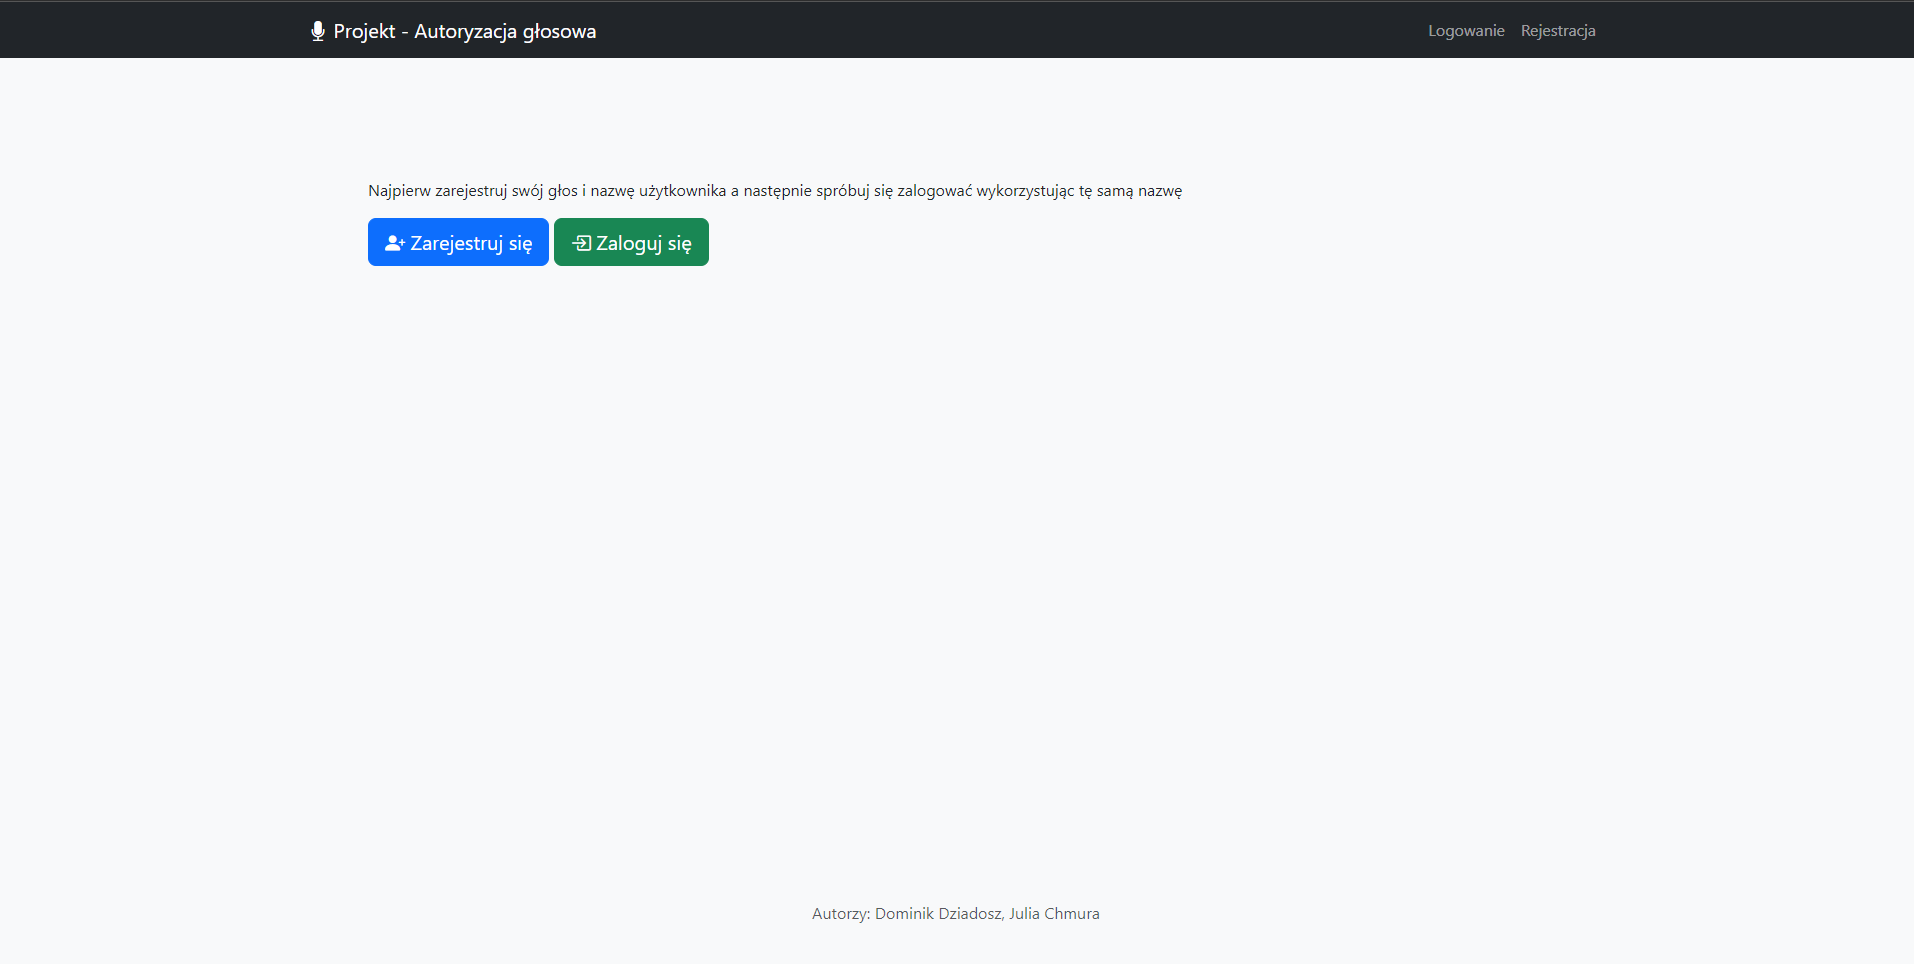
\includegraphics[width=\linewidth]{src/images/strona_glowna.png}
	\caption{Obraz strony głównej}
\end{figure}

Po kliknięciu "Zarejestruj się" przechodzimy do strony rejestracji. Tutaj podawana jest nazwa użytkownika i nagrywana próbka głosu (około 2 do 3 sekundy). 

\begin{figure}[H]
	\centering
	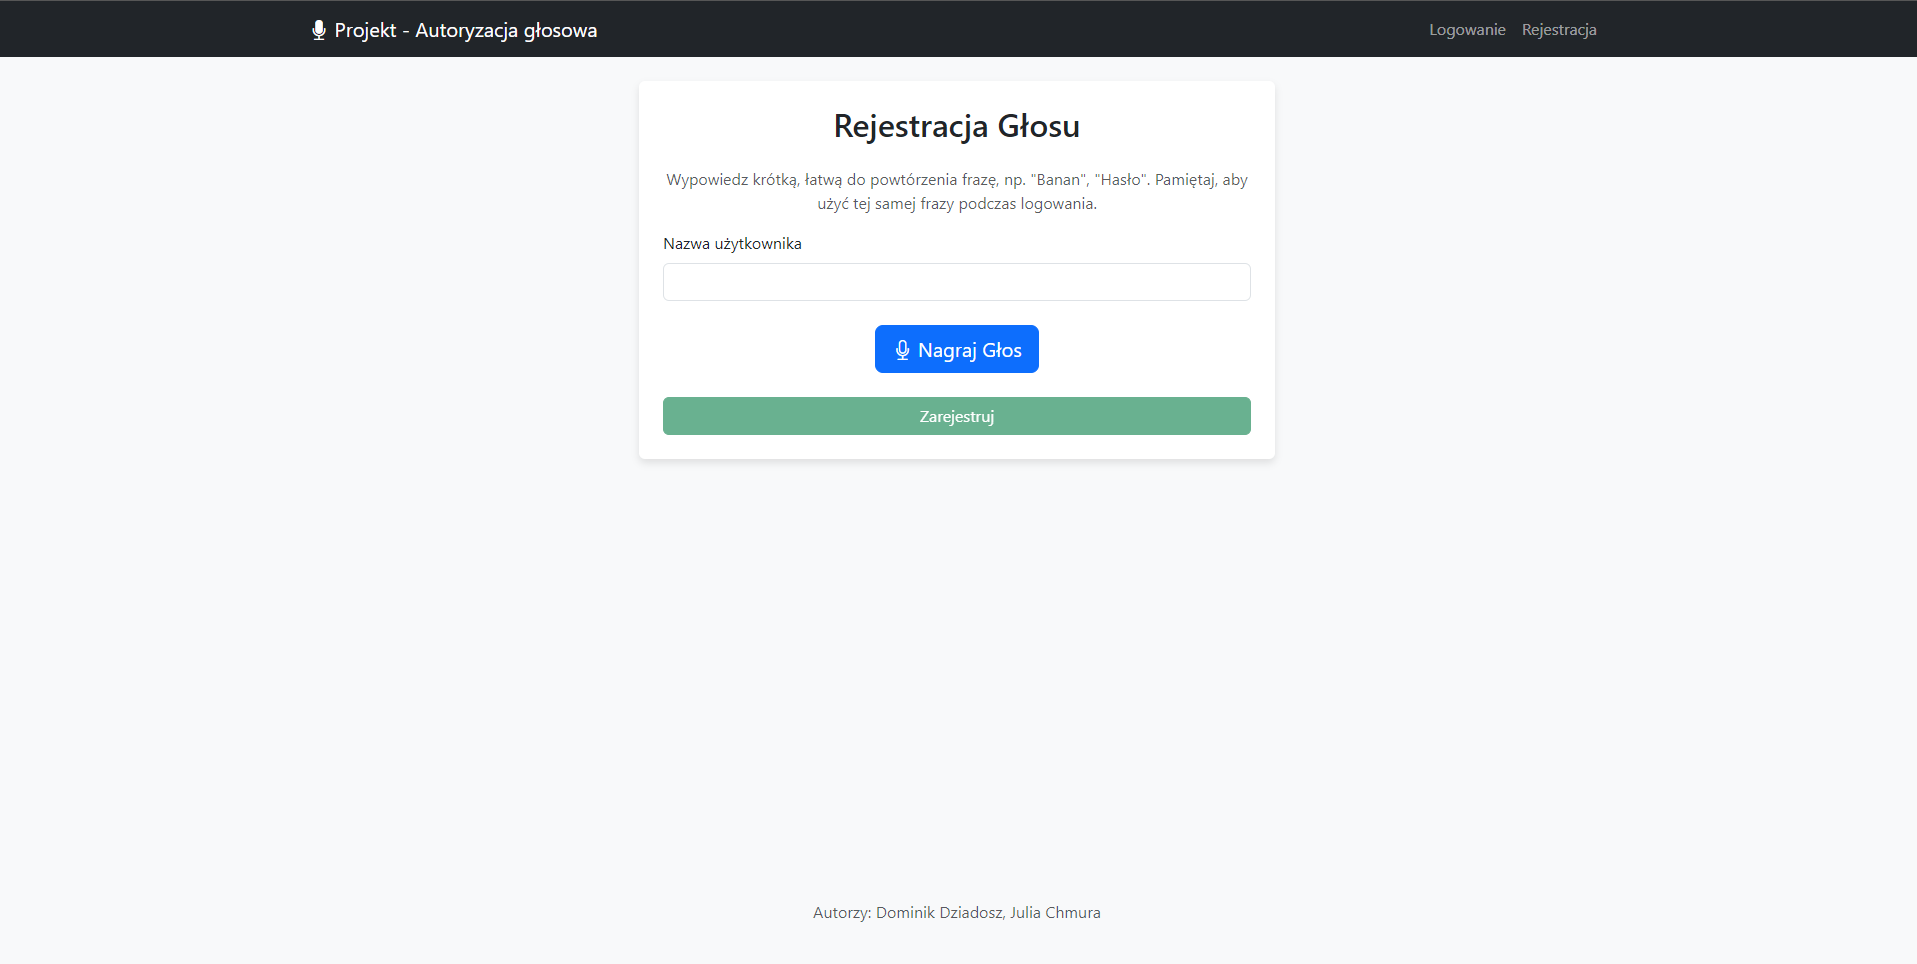
\includegraphics[width=\linewidth]{src/images/nagranie_probki_glosu.png}
	\caption{Obraz strony rejestracji}
\end{figure}

Po zarejestrowaniu się należy przejść do logowania. Tutaj ponownie podajemy nazwę użytkownika i nagrywana jest kolejna próbka, która jest porównywana do tej podanej podczas rejestracji. Jeżeli próbki będą zgodne, użytkownik przechodzi poprawnie przez weryfikację lub nie przechodzi, w każdym przypadku zostaje o tym poinformowany stosownym komunikatem. 

\begin{figure}[H]
	\centering
	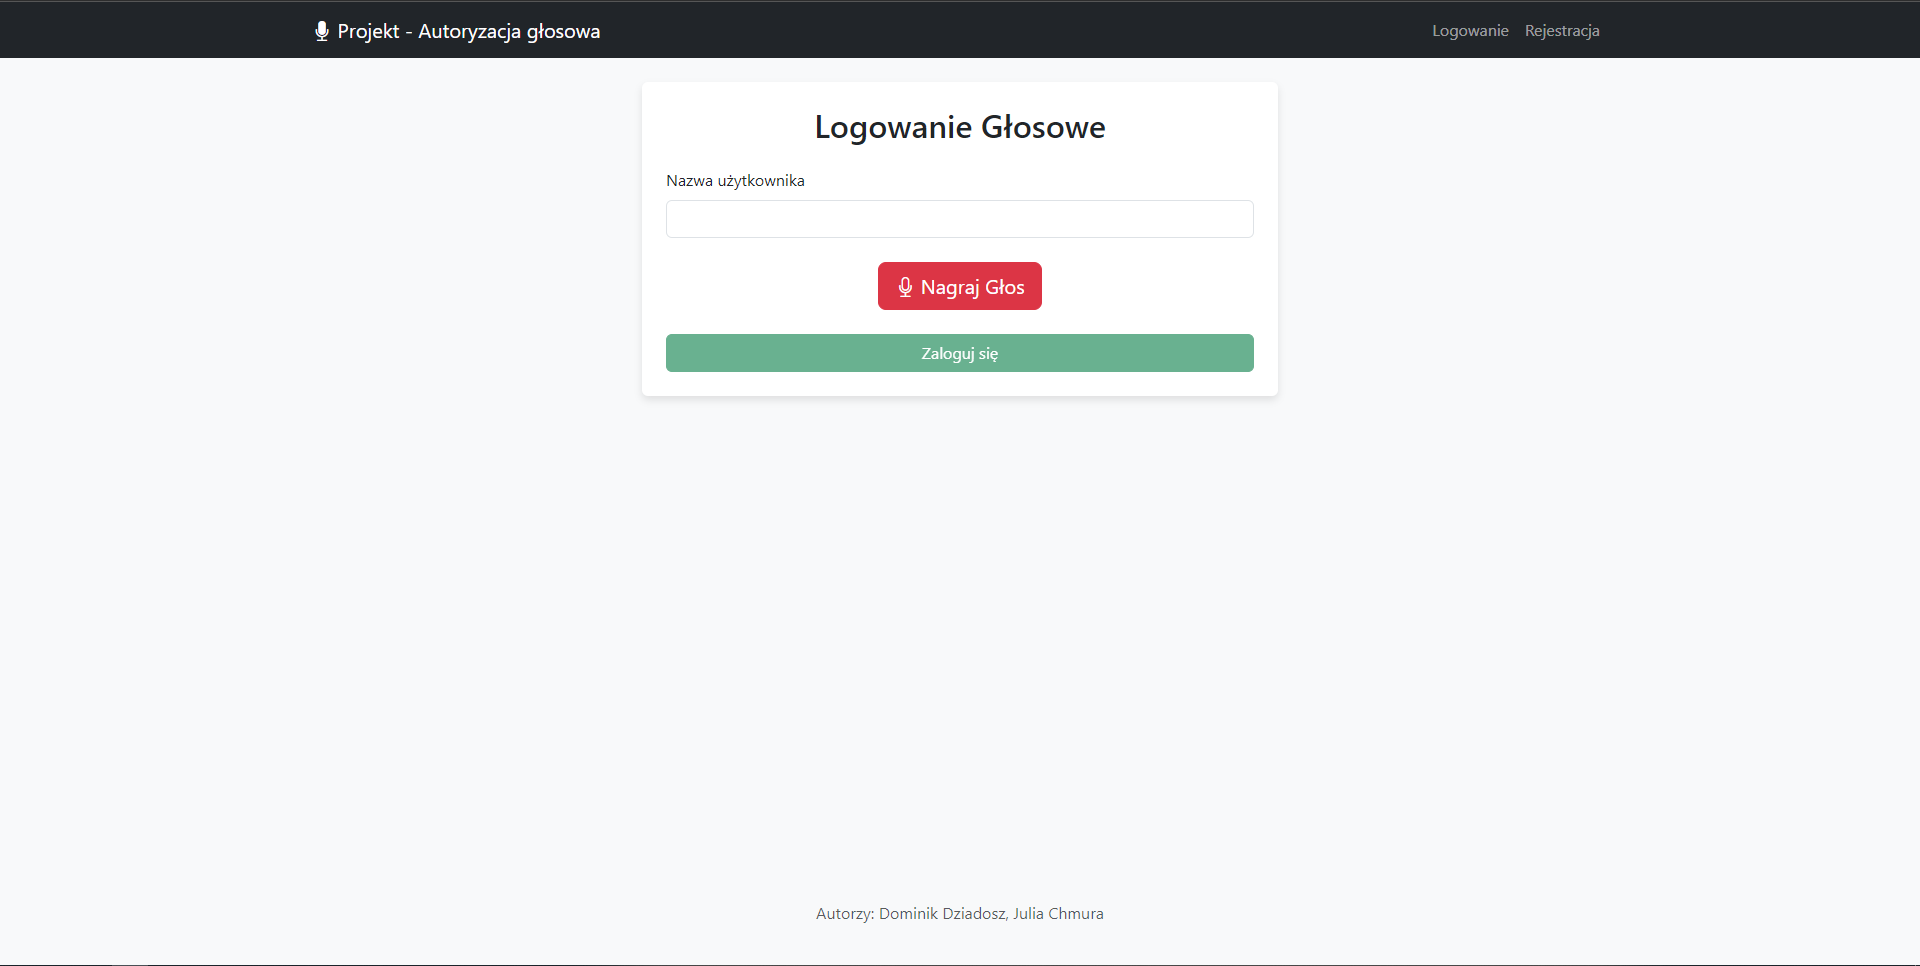
\includegraphics[width=\linewidth]{src/images/weryfikacja_probki_glosu.png}
	\caption{Obraz strony logowania}
\end{figure}

\section{Instrukcja nagrywania próbki głosu}
Aby poprawnie nagrać próbkę głosu należy spełnić dane warunki:
\begin{itemize}
	\item Przygotować odpowiedni sprzęt: poprawnie działający mikrofon
	\item Mówić jednolitym tonem 
	\item Wypowiedzieć proste hasło, najlepiej zkładające się z dwóch słów
	\item Przy rejestracji i logowaniu posłużyć się tym samym zwrotem, mówiąc w takim samym tonie i tempie
	\item Upewnić się że nagrania nie zakłucają odgłosy z otoczenia
	\item Nagrać próbkę trwającą około dwie lub trzy sekundy
	
\end{itemize}


\section{Wnioski}
Na podstawie przeprowadzonych eksperymentów można stwierdzić, że:
\begin{itemize}
    \item Histogram jest przydatnym narzędziem w analizie jakości obrazu biometrycznego.
    \item Wyrównanie histogramu poprawia kontrast i może zwiększać czytelność obrazu.
    \item Segmentacja oparta na histogramie, w szczególności metoda Otsu, pozwala na skuteczne wydzielenie istotnych cech obrazu.
\end{itemize}

\section{Bibliografia}
\begin{itemize}
    \item MATLAB Image Processing Toolbox Documentation \cite{mathworks},
    \item Rafael Gonzalez, Richard Woods, Digital Image Processing Global Edition \cite{gonzalez2017}.
    \item Flask Documentation. Pallets.  \cite{flask_docs}
    \item Pydub Documentation. Read the Docs.  \cite{pydub_docs}
    \item Librosa Documentation  \cite{librosa_docs}
    \item SciPy Documentation  \cite{scipy_docs}
    \item NumPy Documentation \cite{numpy_docs}
    \item scikit-learn Documentation  \cite{scikitlearn_docs}
    \item FFmpeg Documentation  \cite{ffmpeg_docs}
    
\end{itemize}
